\documentclass{article}

% Language setting
% Replace `english' with e.g. `spanish' to change the document language
\usepackage[english]{babel}

% Set page size and margins
% Replace `letterpaper' with `a4paper' for UK/EU standard size
\usepackage[letterpaper,top=2cm,bottom=2cm,left=3cm,right=3cm,marginparwidth=1.75cm]{geometry}

% Useful packages
\usepackage{enumerate}
\usepackage[shortlabels]{enumitem}
\usepackage{amsmath, amsfonts, amssymb, mathtools, stackengine}
\usepackage{graphicx}
\usepackage[colorlinks=true, allcolors=blue]{hyperref}
\usepackage[table]{xcolor}  % For coloring rows
\usepackage{ tipa }
\usepackage[section]{placeins}
\usepackage{float} % For 'H' option of images

% For drawing state machine
\usepackage{tikz}
\usetikzlibrary{automata} % Import library for drawing automata
\usetikzlibrary{positioning} % ...positioning nodes
\usetikzlibrary{arrows} % ...customizing arrows
\tikzset{
    node distance=3cm, % Minimum distance between two nodes. Change if necessary.
    every state/.style={ % Sets the properties for each state
        thick,
        fill=gray!10
    },
    initial text={}, % No label on start arrow
    double distance=2pt, % Adjust appearance of accept states
    bend angle=15,
    every edge/.style={ % Sets the properties for each transition
        draw,
        ->,>=stealth, % Makes edges directed with bold arrowheads
        auto,
        thick
    }
}
            
\let\epsilon\varepsilon

\newcommand{\N}{\mathbb{N}}

\title{
Cyber Physical Systems - Discrete Models \\
[0.2em]Exercise Sheet 9 Solution
}
\author{
  Alper Ari\\
  \texttt{aa508@uni-freiburg.edu}
  \and
  Onur Sahin\\
  \texttt{os141@uni-freiburg.de}
}
\date{\today}

\begin{document}
\maketitle

\section*{Exercise 1:  Safety \& Liveness}

\begin{enumerate}[a]
    \item
    \begin{equation*}
        \begin{split}
            \text{safety} &= \texttt{initially a}\\
            &= \{ A_0 A_1 ... \in (2^{AP})^\omega | a \in A_0 \} \\
            \text{liveness} &= \texttt{eventually a happens} \\
            &= \{ A_0 A_1 ... \in (2^{AP})^\omega | \exists i \in \N \cdot a \in A_i \} \\
        \end{split}
    \end{equation*}

    \item
    \begin{equation*}
        \begin{split}
            \text{safety} &= \texttt{a never happens}\\
            &= \{ A_0 A_1 ... \in (2^{AP})^\omega | \forall i \in \N \cdot a \notin A_i \} \\
            \text{liveness} &= \texttt{eventually a happens infinitely often} \\
            &= \{ A_0 A_1 ... \in (2^{AP})^\omega | \exists ^\infty i \in \N \cdot a \in A_i \}
        \end{split}
    \end{equation*}

    \item
    \begin{equation*}
        \begin{split}
            \text{safety} &= \texttt{initially a}\\
            &= \{ A_0 A_1 ... \in (2^{AP})^\omega | a \in A_0 \} \\
            \text{liveness} &= \textit{such liveness property doesn't exist} \\
            &= \textit{because for every liveness property it holds } \text{pref(E)}=(2^{AP})^*\\
            &= \textit{hence any finite prefix can be extended to satisfy property E} \\
            &= \textit{one needs to check the trace as a whole to ensure it does not satisfy E}
        \end{split}
    \end{equation*}

    \item
    \begin{equation*}
        \begin{split}
            \text{safety} &= \textit{such safety property doesn't exist} \\
            &= \textit{because safety properties have bad prefixes} \\
            &= \textit{thus, it is sufficient to check prefixes of traces } \\
            &= \textit{to ensure it does not satisfy E} \\
            \text{liveness} &= \texttt{eventually a happens infinitely often}\\ 
            &= \{ A_0 A_1 ... \in (2^{AP})^\omega | \exists ^\infty i \in \N \cdot a \in A_i \}
        \end{split}
    \end{equation*}
\end{enumerate}

\newpage
\section*{Exercise 2: Safety-Liveness Decomposition}

\begin{enumerate}[a]
    \item 
    \begin{equation*}
        \begin{split}
            P_{\text{safe}}^{(1)} &= cl(P_1) = P_1 = \{ A_0 A_1 ... \in (2^{AP})^\omega | \forall i \in \N \cdot (a \in A_i \longrightarrow b \in A_{i+1}) \}  \\
            P_{\text{live}}^{(1)} &= P_1 \cup [(2^{AP})^\omega \setminus P_1] = (2^{AP})^\omega = \{A_0 A_1 ... \in (2^{AP})^\omega | true\}\\
        \end{split}
    \end{equation*}
    
    \item 
    \begin{equation*}
        \begin{split}
            P_{\text{safe}}^{(2)} &= cl(P_2) = (2^{AP})^\omega = \{A_0 A_1 ... \in (2^{AP})^\omega | true\} \\
            P_{\text{live}}^{(2)} &= P_2 \cup [(2^{AP})^\omega \setminus P_2] = P_2 = \{A_0 A_1 ... \in (2^{AP})^\omega | \forall i \in \N \cdot \exists j \in \N \cdot (j > i \wedge a \in A_j)\}\\
        \end{split}
    \end{equation*}
    
    \item 
    \begin{equation*}
        \begin{split}
            P_{\text{safe}}^{(3)} &= cl(P_3) = \{A_0 A_1 ... \in (2^{AP})^\omega | \hspace{3mm} |\{i \in \N | a \in A_i\}| \leq 3 \}\\
            P_{\text{live}}^{(3)} &= \stackengine{\baselineskip}{\{A_0 A_1 ... \in (2^{AP})^\omega | \hspace{3mm} |\{i \in \N | a \in A_i\}| = 3 \} \bigcup}{\{A_0 A_1 ... \in (2^{AP})^\omega | \hspace{3mm} |\{i \in \N | a \in A_i\}| > 3 \}}{U}{r}{F}{F}{L}\\
            &= \{A_0 A_1 ... \in (2^{AP})^\omega | \hspace{3mm} |\{i \in \N | a \in A_i\}| \geq 3 \}
        \end{split}
    \end{equation*}
    
    \item 
    \begin{equation*}
        \begin{split}
            P_{\text{safe}}^{(4)} &= cl(P4) = \{ A_0 A_1 ... \in (2^{AP})^\omega | a \in A_0 \}\\
            P_{\text{live}}^{(4)} &=  \stackengine{\baselineskip}{\{ A_0 A_1 ... \in (2^{AP})^\omega | a \in A_0 \wedge \forall i \in \N \cdot \exists j \in \N \cdot (j>i \wedge a \in A_j) \} \hspace{2mm} \bigcup\hspace{2mm} }{\{ A_0 A_1 ... \in (2^{AP})^\omega | a \notin A_0 \}}{U}{r}{F}{F}{L} \\
            &= \{ A_0 A_1 ... \in (2^{AP})^\omega | (a \in A_0 \wedge \forall i \in \N \cdot \exists j \in \N \cdot (j>i \wedge a \in A_j)) \vee (a \notin A_0) \}
        \end{split}
    \end{equation*}
    
    \item 
    \begin{equation*}
        \begin{split}
            P_{\text{safe}}^{(5)} &= cl(P_5) = P_5 = \{ A_0 A_1 ... \in (2^{AP})^\omega | true \}\\
            P_{\text{live}}^{(5)} &= P_5 \cup [(2^{AP})^\omega \setminus P_5] = P_5 = \{ A_0 A_1 ... \in (2^{AP})^\omega | true \}\\
        \end{split}
    \end{equation*}
\end{enumerate}

\newpage
\section*{Exercise 3: Model Checking}

\begin{enumerate}[a)]
    \item \text{}
    \begin{figure}[H]
        \centering
        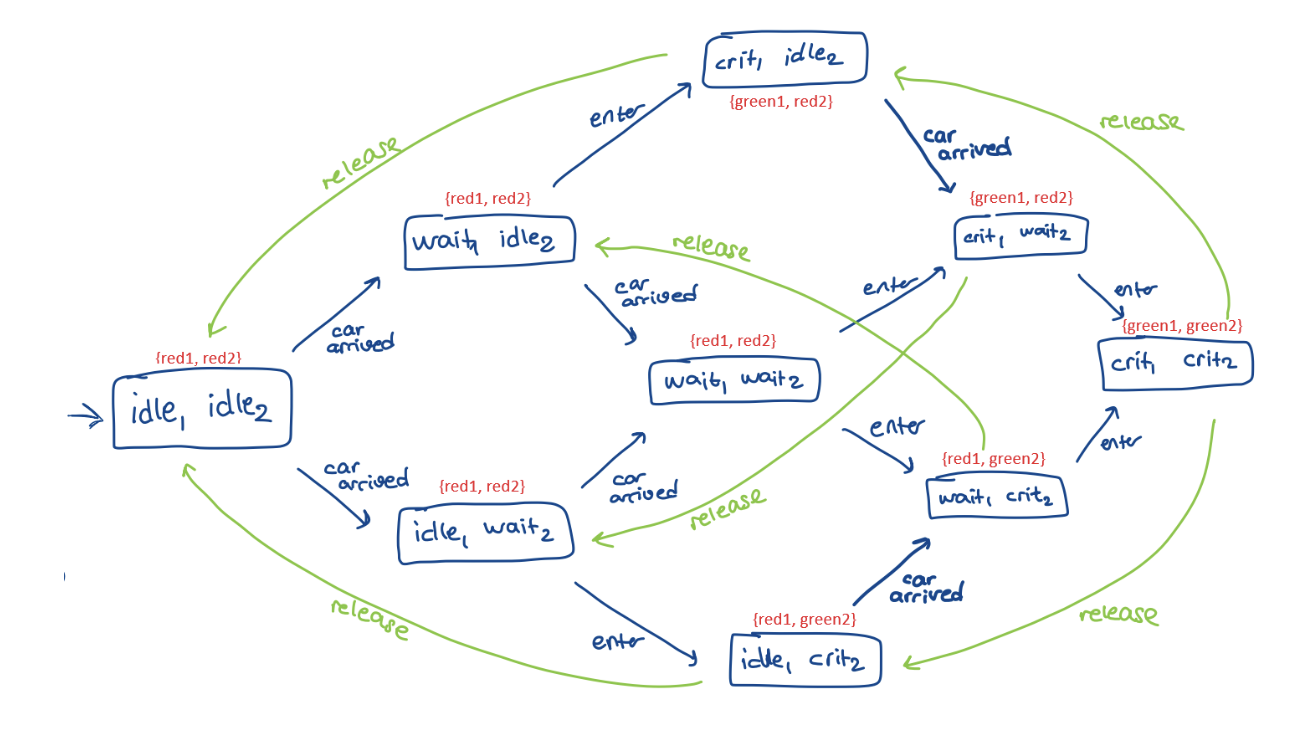
\includegraphics[width=3in]{images/3a.png}
        \caption{\text{NFA $A_T$}}
        \label{fig:3a}
    \end{figure}
    
    \item\text{}
    \begin{figure}[H]
        \centering
        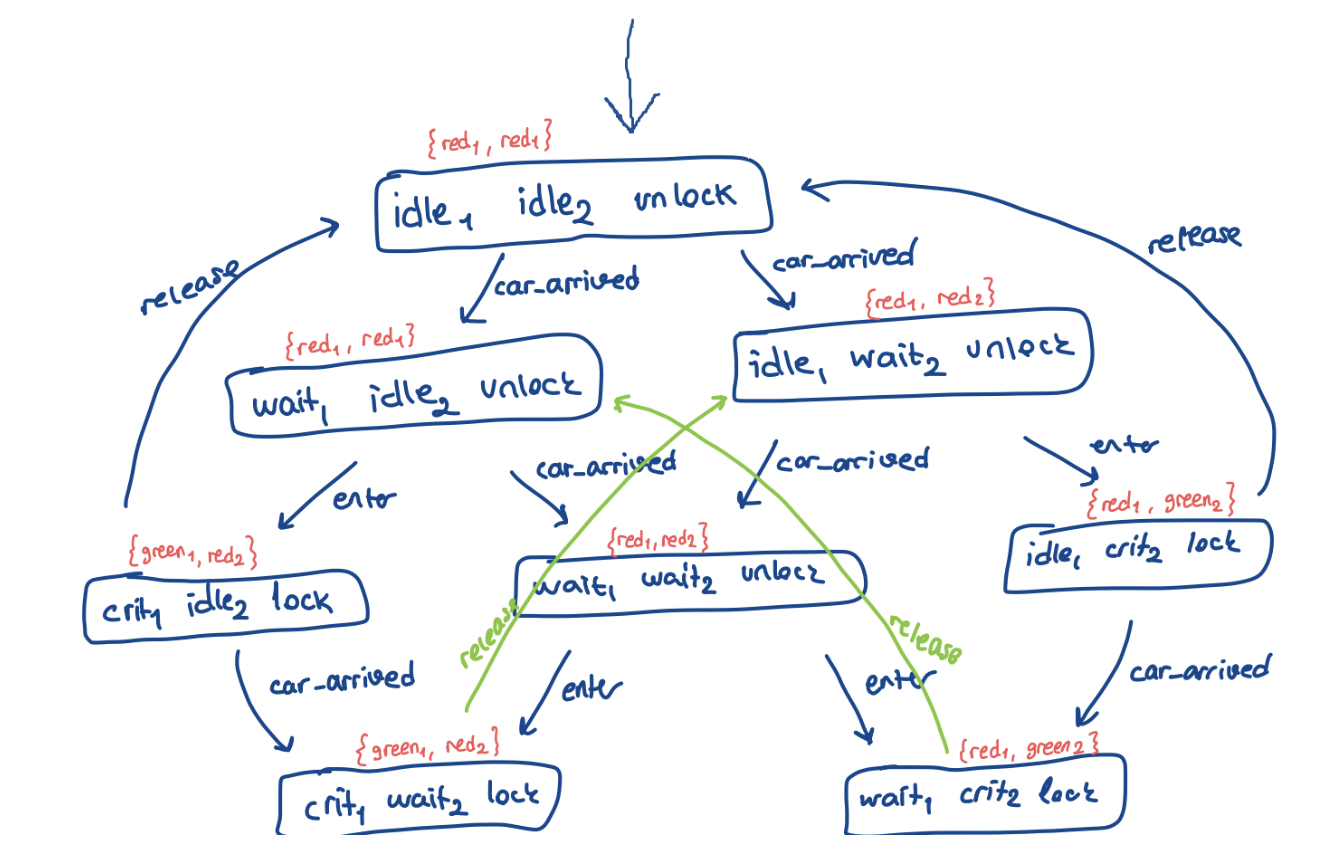
\includegraphics[width=4in]{images/3b.png}
        \caption{\text{NFAs $A_{P_1}$ and $A_{P_2}$}}
        \label{fig:3b}
    \end{figure}

    \item\text{}
    \begin{figure}[H]
        \centering
        \includegraphics[width=4in]{images/3c1.png}
        \caption{\text{\text{Accepting language $A_T \cap A_{P_1}$ is empty, no accepting state is reachable: $T \vDash P_1$}}}
        \label{fig:3c1}
    \end{figure}

    \begin{figure}[H]
        \centering
        \includegraphics[width=4in]{images/3c2.png}
        \caption{\text{\text{Accepting language $A_T \cap A_{P_2}$ is not empty, any accepting state is reachable: $T \nvDash P_2$}}}
        \label{fig:3c2}
    \end{figure}
\end{enumerate}

\end{document}